\documentclass[11pt]{article}
\usepackage[margin=1in]{geometry}
\usepackage[T1]{fontenc}
\usepackage[utf8]{inputenc}
\usepackage{hyperref}
\usepackage{booktabs}
\usepackage{enumitem}
\usepackage{xcolor}
\usepackage{graphicx}

\title{SentinelOps: Verified Technical Review}
\author{Repository Review and Live Validation Pass}
\date{April 11, 2026}

\begin{document}
\maketitle

\begin{abstract}
SentinelOps is now a strong interview-grade and portfolio-grade incident triage system with a credible backend architecture, working operator dashboard, live benchmark path, and a more defensible safety model than the original repository state suggested. This review was not limited to static code reading. The system was rechecked after implementation fixes, database migration alignment, live API validation, benchmark execution, 3D benchmark artifact generation, and Streamlit startup verification. The result is clear: SentinelOps is useful and technically interesting, but it is still a serious prototype rather than a bank-ready production platform. Its real strength is explainable decision support for incident responders in small to medium curated environments, not autonomous remediation at enterprise scale. The latest multi-scenario benchmark shows that the root-cause ranker is now much stronger across scenario families, but model-path stability under sustained benchmark load is still a real bottleneck.
\end{abstract}

\section{What Was Verified}
This pass included both repository review and live runtime validation.

\subsection{Repository and Build Checks}
\begin{itemize}[leftmargin=*]
\item Application, dashboard, eval, and test code compile cleanly under Python 3.12.
\item The project now packages correctly for editable installs after explicit setuptools package discovery was added.
\item Hidden and gitignored proof artifacts were rechecked: tests, eval outputs, \texttt{.env.example}, and \texttt{AGENT.md} are present.
\item The repository includes a multi-scenario simulator, Streamlit dashboard, evaluation harness, Alembic migrations, approval workflows, and audit logging.
\end{itemize}

\subsection{Live Runtime Validation}
The following runtime behaviors were verified directly against a working local deployment:
\begin{itemize}[leftmargin=*]
\item FastAPI started successfully with database connectivity confirmed.
\item The detailed health endpoint returned \texttt{status=ok}, database health \texttt{ok}, 44 indexed runbook chunks, and clean LLM breaker state.
\item A live ingest request completed successfully through grouping, root-cause ranking, runbook retrieval, policy evaluation, and approval creation.
\item The returned incident included non-null \texttt{runbook\_data}, \texttt{policy\_data}, \texttt{pipeline\_metrics}, and \texttt{approval\_request}.
\item A live benchmark run through \texttt{eval/run\_eval.py} completed successfully and produced valid benchmark summaries and figures.
\item Streamlit launched successfully and served HTTP 200 on a local verification port.
\end{itemize}

\section{What Was Fixed During Validation}
Several issues surfaced only during live exercise and were corrected.

\subsection{Operational and Runtime Fixes}
\begin{itemize}[leftmargin=*]
\item Running \texttt{python main.py} and \texttt{uvicorn sentinelops.main:app} from different working directories now works after import-path handling was hardened.
\item Configuration loading now resolves \texttt{.env} from the repository root instead of depending on the current shell directory.
\item The grouping client no longer hard-fails on Gemini models that reject JSON mode. It now retries without \texttt{response\_mime\_type} when needed.
\item Editable install packaging was fixed by explicitly packaging only \texttt{sentinelops*} and including runbook assets.
\item The latest Alembic migration was required and applied because the running database was missing the new \texttt{pipeline\_metrics} and \texttt{policy\_data} columns.
\item The evaluation CLI path was fixed so \texttt{python eval/run\_eval.py ...} works as a direct script from the repository root.
\end{itemize}

\subsection{Hardening Changes Already Present in Code}
\begin{itemize}[leftmargin=*]
\item LLM grouping and runbook synthesis now use timeouts and circuit breakers.
\item Telemetry preprocessing redacts sensitive strings before LLM-facing payloads are created.
\item Incident responses now expose stage-level timing, analysis method, runbook grounding, and policy metadata.
\item A detailed health endpoint exposes database readiness, runbook inventory, breaker state, and active control settings.
\item Streamlit pages now surface policy status, risk level, stage timings, spike diagnostics, and evaluation breakdowns.
\end{itemize}

\section{What Is Right}
\subsection{Architecture}
The architecture is the best part of the project.
\begin{itemize}[leftmargin=*]
\item Route handlers are thin and most logic sits in services.
\item Preprocessing is deterministic and separated from model calls.
\item Root-cause ranking is not free-form generation; it is graph-based plus historical similarity.
\item Runbook retrieval is grounded in indexed source chunks.
\item Human approval is mandatory before action.
\item Audit history is explicit and reviewable.
\end{itemize}

\subsection{System Design Quality}
SentinelOps does not look like an ``LLM wrapper demo''. It looks like a systems project with AI used narrowly where language understanding helps:
\begin{itemize}[leftmargin=*]
\item grouping noisy telemetry into incident clusters,
\item retrieving runbook evidence from semi-structured documentation,
\item synthesizing grounded next steps,
\item preserving deterministic fallbacks when models fail.
\end{itemize}

\subsection{Interview Value}
This is now a strong project to discuss in interviews because it demonstrates:
\begin{itemize}[leftmargin=*]
\item async backend design,
\item schema evolution with Alembic,
\item AI fallbacks and safety controls,
\item retrieval and graph-based reasoning,
\item dashboarding and evaluation,
\item debugging real deployment issues rather than just training-time ideas.
\end{itemize}

\section{What the Live System Shows}
\subsection{One Verified End-to-End Incident}
The verified live ingest produced:
\begin{itemize}[leftmargin=*]
\item successful LLM grouping without fallback,
\item top cause \texttt{db-primary},
\item analysis method \texttt{graph+vector},
\item grounded runbook retrieval from three source files,
\item policy decision \texttt{RESTRICTED\_REVIEW},
\item approval request \texttt{PENDING},
\item total pipeline time of roughly 17.8 seconds on the validated run.
\end{itemize}

\subsection{One Verified Live Benchmark Run}
The live benchmark produced:
\begin{itemize}[leftmargin=*]
\item success rate: 100\% (1/1),
\item top-1 root-cause accuracy: 100\%,
\item grouping fallback rate: 0\%,
\item runbook grounding rate: 100\%,
\item mean latency: about 21.6 seconds,
\item dominant stage: runbook synthesis.
\end{itemize}

This is not enough to claim broad performance, but it is enough to demonstrate that the evaluation path and graph surfaces are functional.

\subsection{Verified Multi-Scenario Benchmark}
A broader live benchmark was then run across all five scenario families with two runs per scenario, for a total of 10 live executions. The results are more informative than the single-run check because they expose both strengths and weaknesses.

\begin{center}
\begin{tabular}{lr}
\toprule
Metric & Verified result \\
\midrule
Total runs & 10 \\
Successful runs & 10 \\
Overall success rate & 100\% \\
Root-cause top-1 accuracy & 20\% \\
Root-cause top-1 accuracy & 90\% \\
Grouping fallback rate & 80\% \\
Runbook grounding rate & 100\% \\
Expected source hit rate & 100\% \\
Mean latency & 10.29 s \\
P95 latency & 19.04 s \\
Mean pipeline total & 9.66 s \\
Dominant policy status & \texttt{ESCALATE\_REQUIRED} (9/10) \\
\bottomrule
\end{tabular}
\end{center}

This updated benchmark changes the interpretation of the project in an important way. The ranker bias problem was materially improved: live top-1 root-cause accuracy moved from 20\% in the earlier benchmark pass to 90\% after direct-evidence gating and richer incident text were added to the ranking path. The remaining miss occurred on one \texttt{auth\_outage} run, which was misranked as \texttt{cache-service}. At the same time, the benchmark also surfaced a new operational truth: grouping fallback rose to 80\% because the live model path became unstable under sustained benchmark load and opened the configured circuit breakers. That makes the current limitation different from before. The main ranking logic is now much stronger, but LLM-path reliability is still a serious runtime concern.

\section{What Problems It Solves}
The project solves a real operations problem: \emph{decision compression during early incident response}. Specifically, it reduces the amount of manual stitching an operator has to do across logs, alerts, topology, past incidents, and runbooks.

\subsection{Useful Outputs}
For a responder, the system turns a telemetry bundle into:
\begin{enumerate}[leftmargin=*]
\item grouped incident hypotheses,
\item a ranked likely root cause,
\item grounded runbook actions,
\item explicit policy and reviewer guidance,
\item auditable approval state.
\end{enumerate}

\subsection{Who It Helps}
It is helpful for:
\begin{itemize}[leftmargin=*]
\item SRE and platform interviews,
\item internal demos and proofs of concept,
\item teams with recurring incident families,
\item environments where human operators need faster triage rather than full automation.
\end{itemize}

\section{What It Does Not Solve Yet}
SentinelOps still does not prove the following:
\begin{itemize}[leftmargin=*]
\item enterprise identity and access control,
\item secrets management and key rotation,
\item multi-tenant isolation,
\item policy enforcement backed by organizational controls,
\item dynamic service topology discovery,
\item large-scale incident history and benchmark diversity,
\item low-latency response suitable for strict operational SLAs.
\end{itemize}

It is also not an autonomous remediation platform. It recommends and escalates; it does not safely execute changes in production.

\section{What the Graphs Mean}
The evaluation visuals are now more informative than before because they expose stage latency, spike attribution, policy state, and scenario-level behavior. The newly added 3D plots are useful because they show how confidence, latency, workload size, and pipeline stages interact across the live benchmark set.

\subsection{Current Interpretation}
The graphs now support these claims:
\begin{itemize}[leftmargin=*]
\item the pipeline stages are measurable end to end,
\item latency spikes can be attributed to a specific stage instead of just observed globally,
\item policy and risk distributions are inspectable,
\item live and committed evaluation outputs share the same schema,
\item multi-scenario results can now be visualized as both run-level and scenario-level 3D artifacts.
\end{itemize}

\subsection{Important Current Signal}
Across the validated multi-scenario benchmark, the most important signals are:
\begin{itemize}[leftmargin=*]
\item the root-cause ranker no longer collapses most non-database incidents back to \texttt{db-primary},
\item the slowest spikes were still driven by \texttt{runbook} synthesis on the \texttt{auth\_outage} scenario,
\item grouping became the unstable component under sustained load, with breaker-triggered fallback dominating later runs,
\item pipeline reliability remained high enough to complete all 10 benchmark executions despite degraded model availability.
\end{itemize}

\begin{figure}[htbp]
\centering
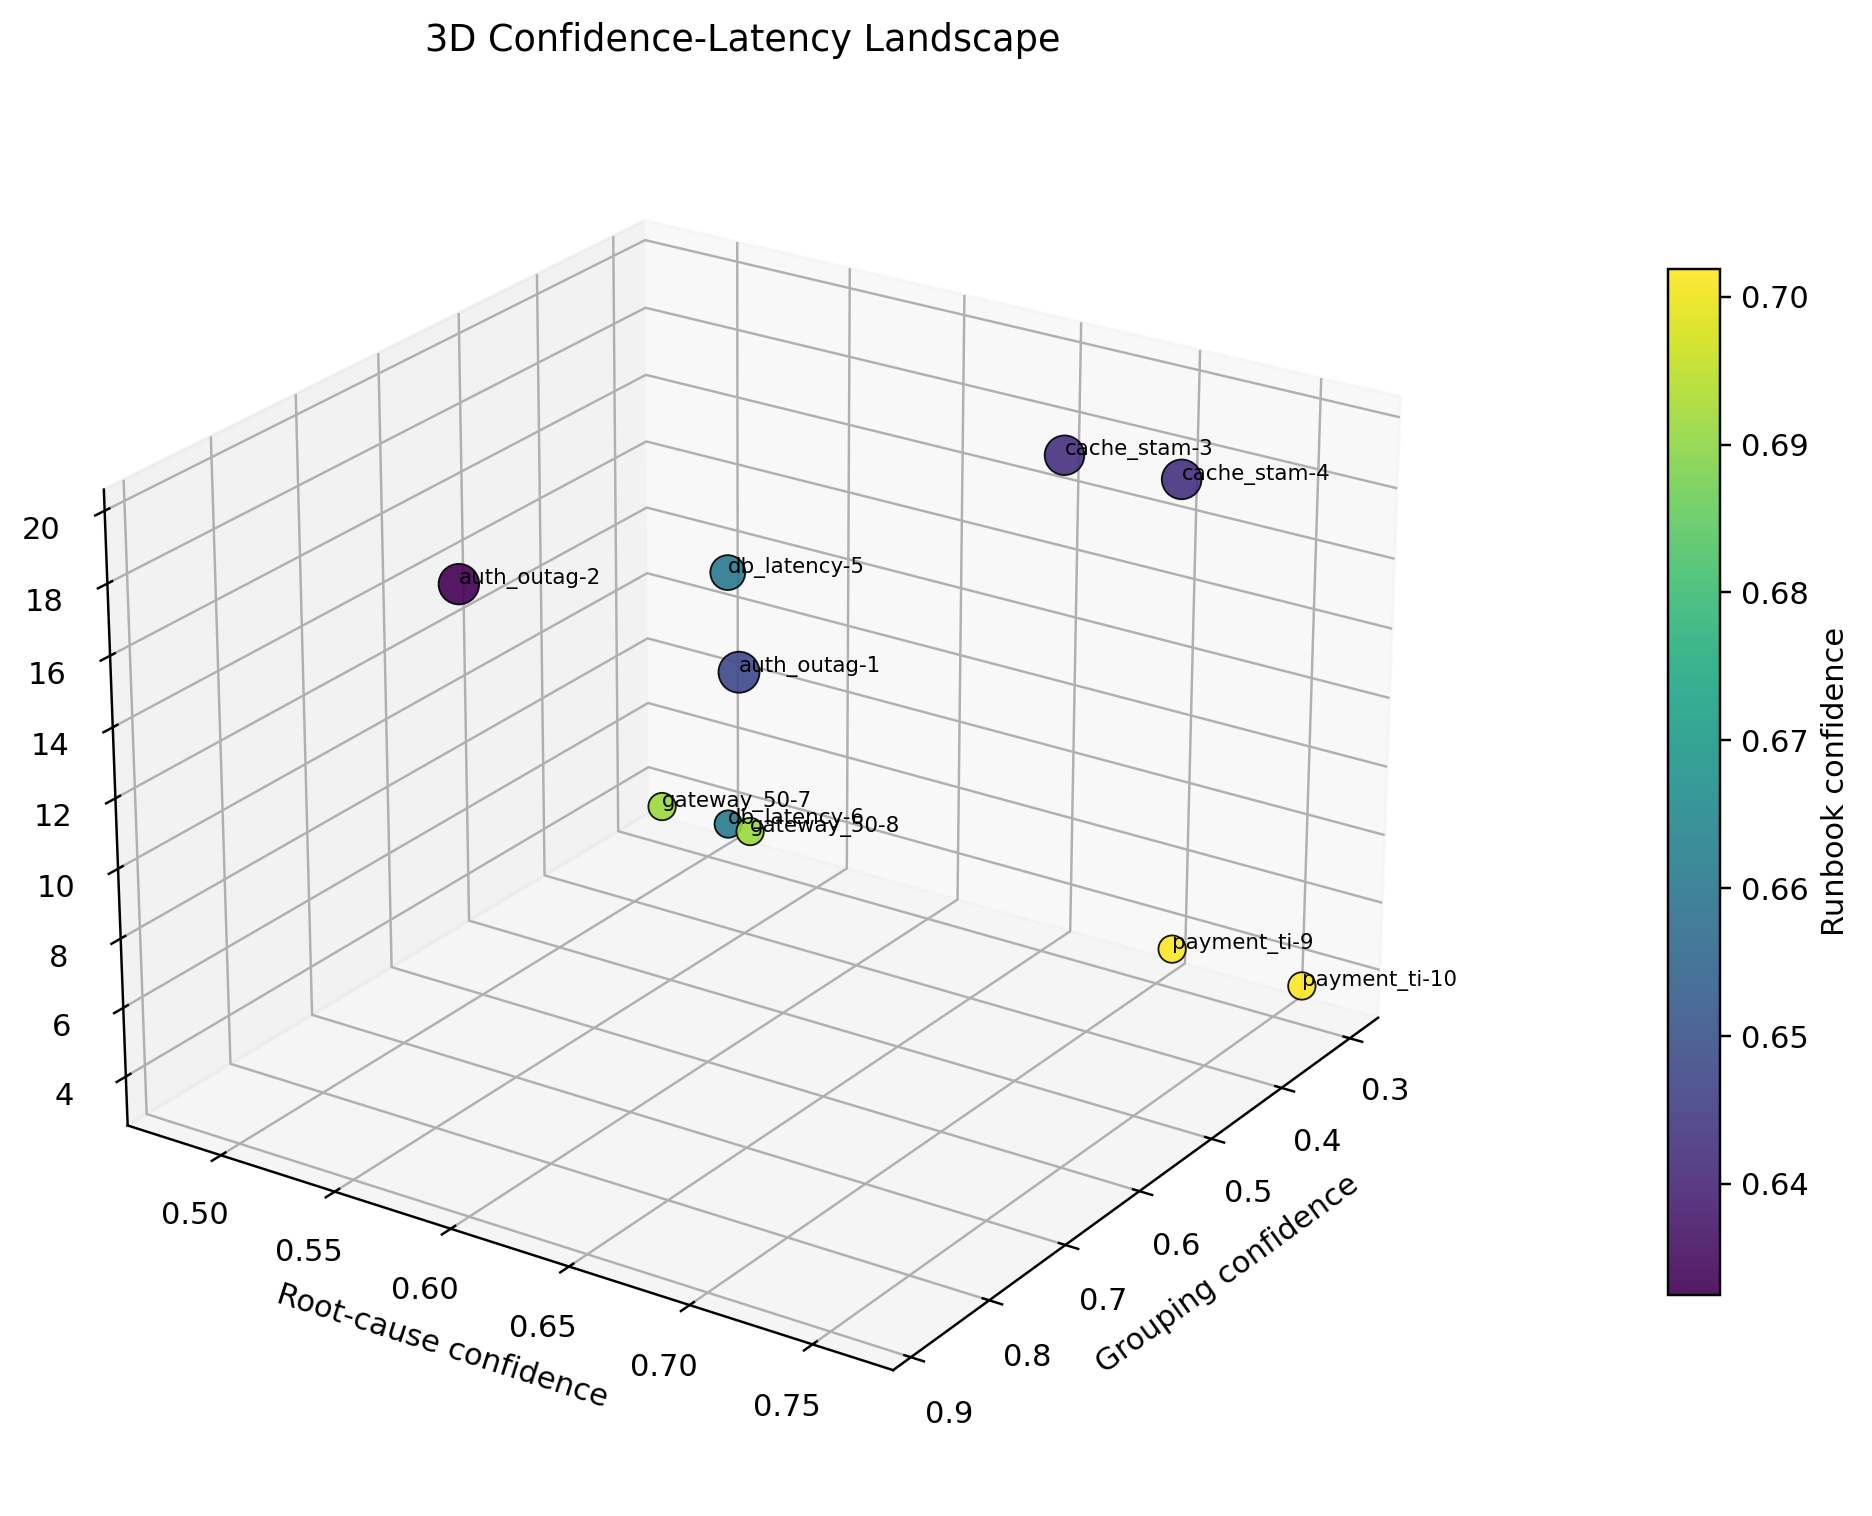
\includegraphics[width=0.82\textwidth]{../eval/results/live_multiscenario_v2/benchmark_3d_confidence_latency.png}
\caption{3D confidence-latency landscape for the live multi-scenario benchmark. Each point is one benchmark run. The plot shows that latency and confidence are not tightly coupled; high-confidence runs can still incur long pipeline times.}
\end{figure}

\begin{figure}[htbp]
\centering
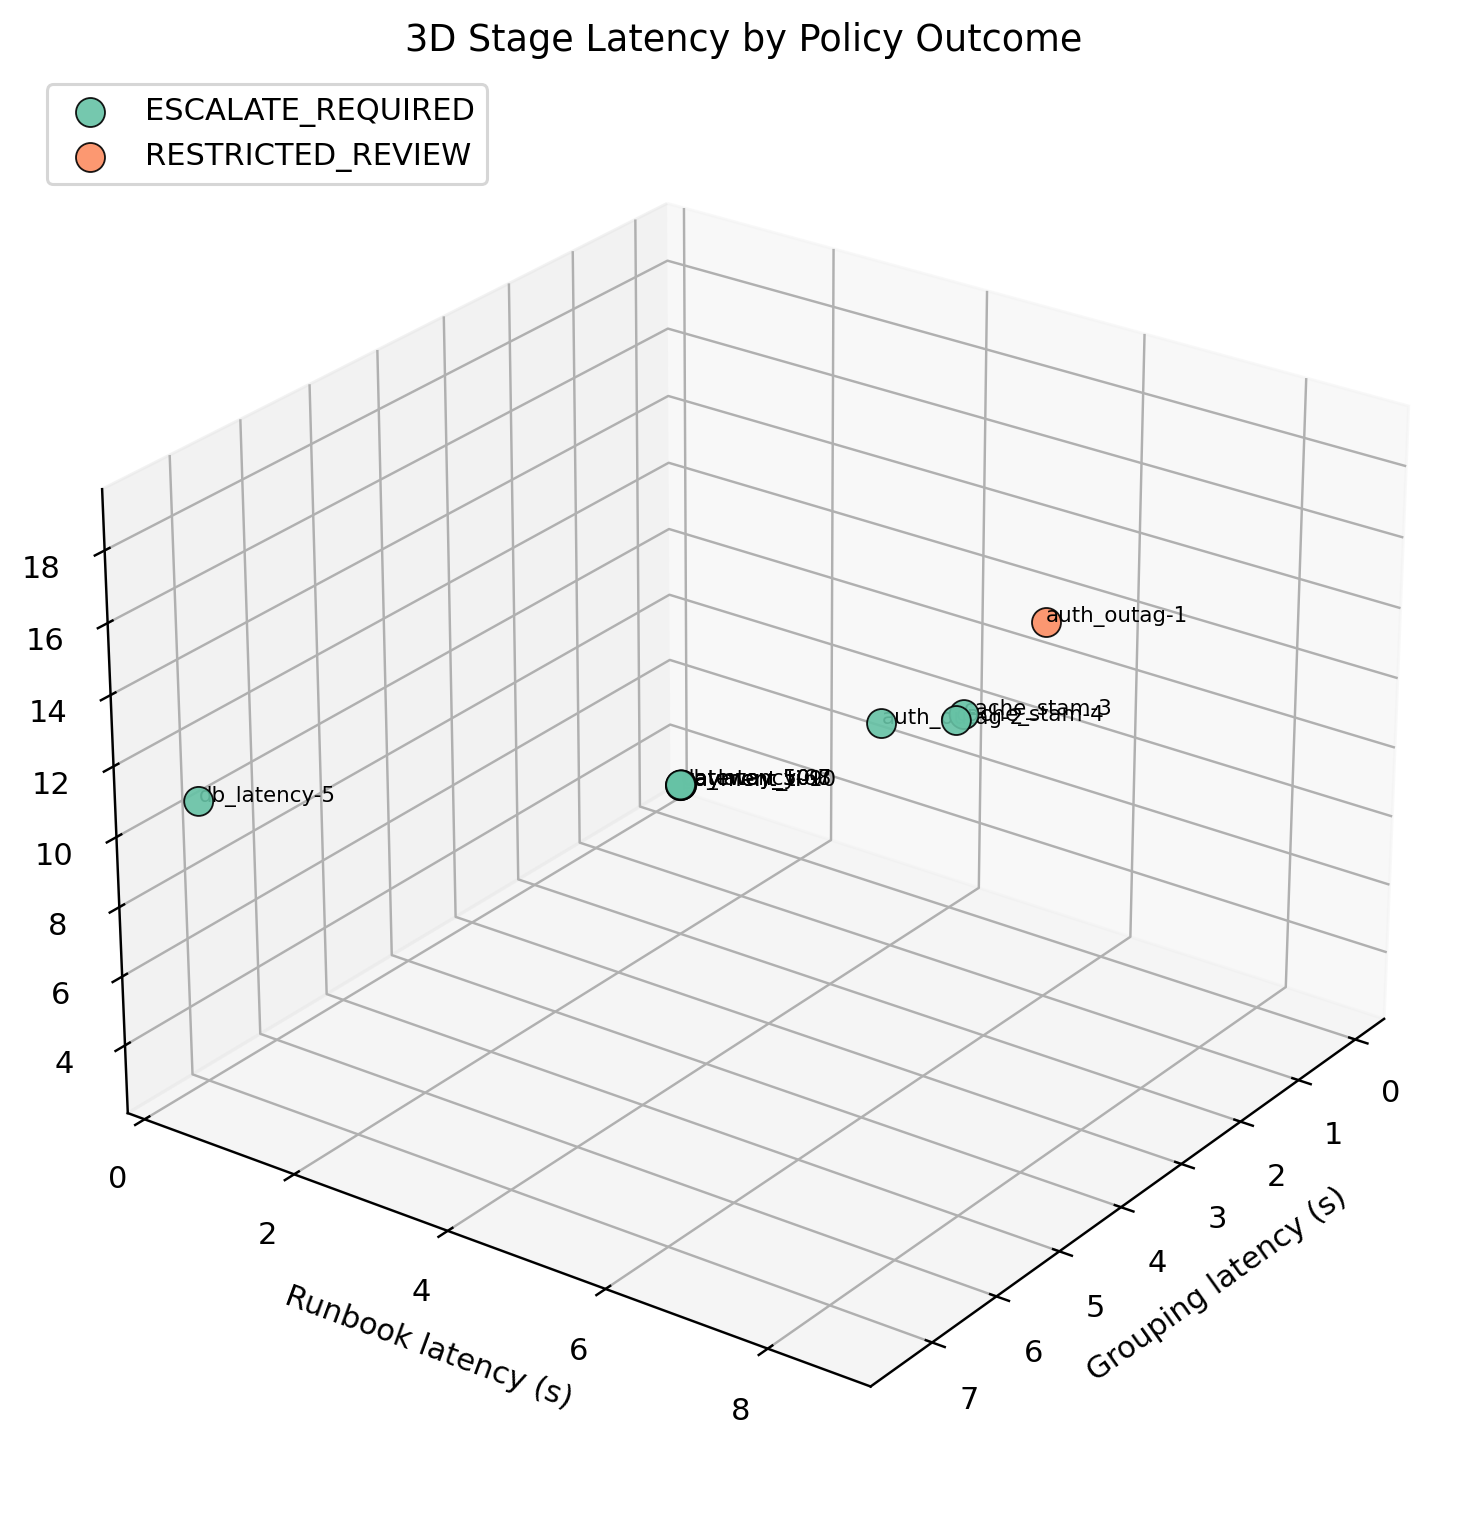
\includegraphics[width=0.82\textwidth]{../eval/results/live_multiscenario_v2/benchmark_3d_stage_latency.png}
\caption{3D stage-latency view of grouping, runbook, and total pipeline time colored by policy outcome. The slowest runs are still runbook-heavy, but the figure also shows how degraded grouping reliability pushes most runs into an escalated review posture.}
\end{figure}

\begin{figure}[htbp]
\centering
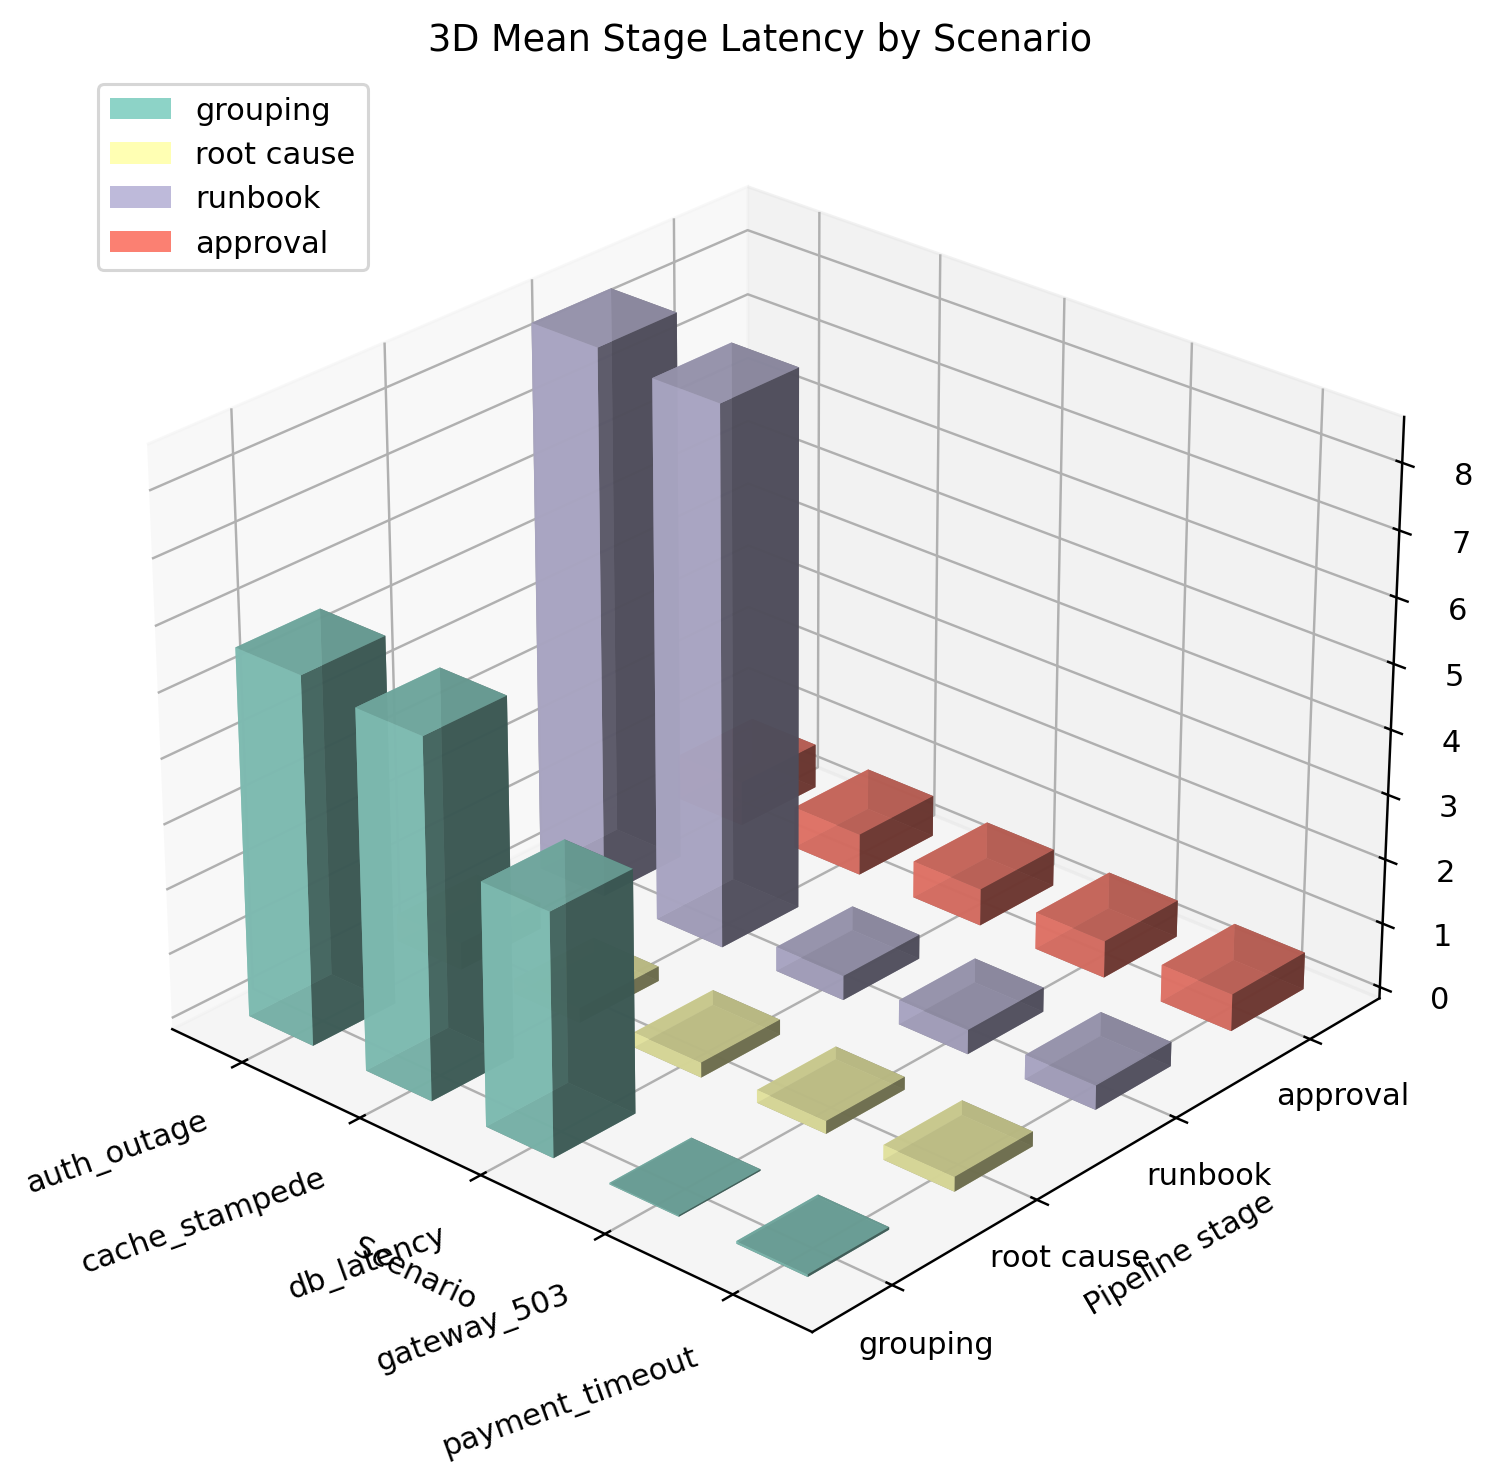
\includegraphics[width=0.82\textwidth]{../eval/results/live_multiscenario_v2/benchmark_3d_scenario_stage_bars.png}
\caption{3D mean stage latency by scenario. This is the most useful optimization plot in the set because it makes stage-level bottlenecks visible by scenario family rather than only by individual run.}
\end{figure}

\section{At What Scale Is It Credible?}
\begin{itemize}[leftmargin=*]
\item \textbf{Credible now:} demo systems, interview presentations, course or capstone projects, and internal pilot environments with curated runbooks and known service graphs.
\item \textbf{Potential with more engineering:} small to medium service estates with recurring incident classes and controlled operator workflows.
\item \textbf{Not yet credible:} actual bank-scale production automation across large, fast-changing, highly regulated systems.
\end{itemize}

The right honest statement is that the approach can be integrated with a bank-style workflow design, but the current implementation is not yet deployable as a bank production control plane.

\section{Should It Be Posted Publicly?}
Yes. It is worth posting, but the framing should be disciplined.

\subsection{Good Positioning}
\begin{itemize}[leftmargin=*]
\item explainable AI incident triage system,
\item human-in-the-loop operational assistant,
\item graph + retrieval + policy backed response workflow,
\item backend systems project with live validation and dashboards.
\end{itemize}

\subsection{Bad Positioning}
\begin{itemize}[leftmargin=*]
\item autonomous incident response,
\item enterprise-ready banking platform,
\item proven universal root-cause AI,
\item production-safe remediation engine.
\end{itemize}

\subsection{Suggested Public Description}
\begin{quote}
SentinelOps is an explainable incident triage system that combines deterministic preprocessing, dependency-graph root-cause ranking, grounded runbook retrieval, policy-based review guidance, and human approval. It now supports live operator workflows, benchmark reporting, and failure-aware controls such as timeouts, breakers, and safe fallbacks.
\end{quote}

\section{Remaining Gaps Before ``Production Grade''}
The highest-value remaining steps are:
\begin{enumerate}[leftmargin=*]
\item CI that actually runs tests and migrations on every change.
\item Auth, RBAC, and approval identity hardening.
\item Structured metrics export to Prometheus/OpenTelemetry rather than dashboard-only views.
\item Better benchmark breadth across more scenario families and cold-start conditions.
\item Faster or cheaper runbook synthesis to reduce end-to-end latency.
\item Dynamic topology ingestion instead of a static graph file.
\item Operational rate limits, quotas, and stronger data-retention controls.
\end{enumerate}

\section{Bottom Line}
SentinelOps now looks good for the right reasons. It has:
\begin{itemize}[leftmargin=*]
\item a coherent architecture,
\item meaningful runtime controls,
\item a working dashboard path,
\item live benchmark capability,
\item and enough real debugging history to make it an excellent interview project.
\end{itemize}

It is not ``all good at everything''. The latest benchmark shows a more nuanced reality: the ranker is now strong enough to discuss seriously, but the model-dependent grouping path is still unstable under sustained benchmark load. That is still a strong result for interview and public presentation because the project now demonstrates both engineering depth and honest measurement. SentinelOps is best presented as a strong, explainable, well-instrumented incident triage prototype with verified runtime controls, markedly improved ranking quality, and clear next optimization targets around LLM reliability.

\end{document}
